\section{Stratégie du point de vue \textsl{commercial}}
\label{sec:monocrit}
Le responsable commercial cherche à équilibrer le nombre
d'unités de ${A, B, C}$ (famille 1) et ${D, E, F}$ (famille 2) afin que ces deux
familles contiennent le même nombre d'unités (à $\epsilon$ unité(s) prés).
~\\
En prennant en compte les contraintes définies plus haut et y en ajoutant une nouvelle
\textbf{contrainte d'équilibre} entre les deux familles de produits, il apparait que
la meilleure solution serait de ne rien produire.\\
Encore une fois, cette solution n'est pas avantageuse.\\
Introduisons par conséquent une autre contrainte : nous allons 
essayer d'équilibrer les familles de produits tout en conservant un bénéfice
maximal. 

\subsection{Modélisation}
Soient :
\begin{itemize}
	\item $n_A$ le nombre de produits A usinés. 
	\item $n_B$ le nombre de produits B usinés. 
	\item $n_C$ le nombre de produits C usinés. 
	\item $n_D$ le nombre de produits D usinés. 
	\item $n_E$ le nombre de produits E usinés. 
	\item $n_F$ le nombre de produits F usinés. 
\end{itemize}
~\\
Pour étudier l'équilibre entre les deux familles des produits on définira une
fonction qui sera égale à la différence entre les quantités des produits
provenant des deux familles, soit: 
\begin{displaymath}
	F = (n_A+n_B+n_C)-(n_D+n_E+n_F)
\end{displaymath}

La contrainte sur l'équilibre va se traduire par l'essai de minimiser la
fonction F, c'est à dire:
\begin{eqnarray*}
	|F| &\leq& \epsilon\\
	\Leftrightarrow -\epsilon \leq F &\leq& \epsilon\\
	\Leftrightarrow -\epsilon \leq (n_A+n_B+n_C)-(n_D+n_E+n_F)
	&\leq& \epsilon\\
	Avec& \epsilon \rightarrow 0.\\
\end{eqnarray*} 

\subsection{Stratégie adoptée}
Comme indiqué plus haut nous allons essayer de trouver le nombre d'unités à produire de telle manière que :
\begin{enumerate}
	\item Les famille 1 et 2 soient équilibrée
	\item Le bénefice soit maximum
\end{enumerate}

Pour cela :
\begin{itemize}
	\item Nous fixons un certain bénéfice à atteindre
	\item Pour le bénéfice choisi, nous essayons de minimiser F. 
\end{itemize}
~\\
Pour rester toujours dans une programmmation monocritère nous répèterons cette
démarche un certain nombre de fois (pour des pourcentages différentes du benefice).\\
Nous pourrons donc tracer une courbe représentant la valeur de F en fonction du bénéfice atteint.\\
~\\
\textbf{L'interprétation de cette courbe nous permettra de trouver le 
meilleur compromis.}\\
~\\
Pour s'approcher de l'équilibre nous utilisons la fonction linprog de Matlab de la
manière suivante:\\
\addCode{../SourcesMatlab/commercialSnippet.m}{matlab}
~\\
F correspond à la fonction qu'on essaie de minimiser.
\texttt{[infEqConstraints;-Earnings]} et \texttt{[infEqValues;-b]} sont les matrices qui
modelisent la prise en compte de toutes les contraintes générales auxquelles on
a ajouté la contrainte de s'approcher d'un certain benefice. Pour obtenir une
valeur de F qui s'approche de 0 nous effectuerons deux appels de linprog:\\
un en utilisant la fonction F et un en utilisant la fonction -F. Les contraintes
restent les mêmes pour les deux appels.\\
~\\
Le graphe suivant est obtenu :
\begin{figure}[h!]
	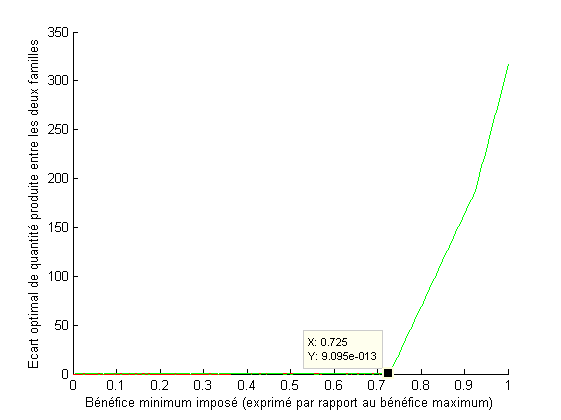
\includegraphics[width=\textwidth]{../SourcesMatlab/graphe_resp_commercial_petit.png}
\end{figure}

La courbe verte correspond aux valeurs minimales de F, la courbe rouge les
valeurs minimales de -F.\\
On observe dès le début qu'on peut approcher les deux courbes de $0$ différentes valeurs du benefice.
Autrement dit, il est possible d'avoir un équilibre des benefices respectifs. Au bout d'un moment, les deux courbes
commencent à s'écarter et l'équilibre est rompu.\\
~\\
C'est au point de rupture qu'est le meilleur rapport entre les deux
contraintes (l'équilibre et le benefice obtenu).\\
\textbf{Le meilleur compromis est donc obtenu autour de 72.5\% du benefice maximum.}\\
L'écart entre les deux familles de produits est : $9.095*10^{-13}$ ce qui est tres proche de 0 
et donc en conformité avec notre objectif.\\
~\\ 
Les quantités de production pour chaque produit sont les suivantes:
\begin{itemize}
	\item $n_A$ = 0,8888
	\item $n_B$ = 114,9102
	\item $n_C$ = 60,2321
	\item $n_D$ = 0,2537
	\item $n_E$ = 148,7430
	\item $n_F$ = 27,0343
\end{itemize}
~\\
\begin{center}
	\fbox{\textbf{Le benefice obtenu est de 7646,575 unités monétaires.}}
\end{center}
